\documentclass[12pt, oneside, openany]{article}
\usepackage[T1]{fontenc}
\usepackage[spanish, es-tabla, es-lcroman]{babel}
\usepackage[utf8]{inputenc}
\usepackage[document]{ragged2e}
\usepackage{tcolorbox}
\tcbuselibrary{theorems}
\usepackage{cancel}
\usepackage{amssymb}
\usepackage{amsmath}
\usepackage{mathrsfs}
\usepackage{wrapfig}
\usepackage{fancyhdr}
\usepackage{colortbl}
\usepackage{graphicx}
\usepackage{subcaption}
\usepackage{xcolor}
\usepackage{tikz}
\usepackage{multicol}
\usepackage{multirow}
\usepackage{lastpage}
\usepackage{pdfpages}
\usepackage{listings}
\usepackage{blindtext}
\spanishdecimal{.}
\usepackage[explicit]{titlesec}
\usepackage[colorlinks=true, linkcolor=black, citecolor=black, urlcolor=blue]{hyperref}
\usepackage[a4paper, total={16cm, 24cm}]{geometry}
\pagestyle{fancy}
\lhead{Muñoz Nuñez Ian Emmanuel}
\rhead{Proyecto 2}
\lfoot{Mtra. María Patricia Ventura Nuñez}
\rfoot{CUCEI}
\renewcommand{\headrulewidth}{1pt}
\renewcommand{\footrulewidth}{1pt}

\begin{document}

\begin{titlepage}
    \pagenumbering{roman}
    \centering
    {\bfseries\LARGE Universidad de Guadalajara \par}
    \vfill
    {
        \includegraphics[width=0.3\linewidth]{UdG.png}
        \includegraphics[width=0.3\linewidth]{qci.png}
        \par
    }
    \vfill
    {\bfseries\LARGE Seminario de problemas de programación de sistemas reconfigurables \par}
    \vfill
    {\bfseries\LARGE Proyecto 2 \par}
    \vfill
    {\LARGE Diseño de un circuito combinacional que genere un bit de paridad impar, utilizando compuertas \emph{or exclusivas} y/o \emph{nor exclusiva} \par}
    \vfill
    {\bfseries\LARGE Nombre: \par}
    \vfill
    {\bfseries\LARGE Muñoz Nuñez Ian Emmanuel \par}
    \vfill
    {\bfseries\LARGE Sección: D01 \par}
    \vfill
    {\bfseries\LARGE Código: 216464457 \par}
    \vfill
    {\bfseries\LARGE Maestra: \par}
    \vfill
    {\bfseries\LARGE María Patricia Ventura Nuñez \par}
    \vfill
    {\bfseries\LARGE Ingeniería robótica \par}
\end{titlepage}

\pagenumbering{arabic}
\newpage

\section{Objetivo}
{\sffamily\Large
    \hspace{0.5cm} Solucionar problemas de diseño utilizando las herramientas aprendidas en \emph{Programación de Sistemas Reconfigurables}.
    
    \hspace{0.5cm} Utilizar hojas de datos de las familias lógicas.
    
    \hspace{0.5cm}Simular circuitos digitales en programas de diseño como \emph{Proteus\texttrademark} e implementarlos físicamente.
    
    \hspace{0.5cm} Diseñar e implementar una función utilizando compuertas \emph{orex} y \emph{norex}. Por ejemplo:
    
    \renewcommand{\labelitemi}{-}
    \begin{itemize}
        \item Un detector de paridad par y/o impar.
        \item Un sumador o restador de 4 bits.
    \end{itemize}
    
}

\section{Material}
{\sffamily\Large
    \renewcommand{\labelitemi}{$\bullet$}
    \begin{itemize}
        \item Protoboard.
        \item Fuente VCC (5V).
        \item Led verde.
        \item Resistencias de 200$\Omega$ y 2$k\Omega$.
        \item 1 dip switch de 8 bits.
        \item 1 display de 7 segmentos.
        \item 1 barra de leds de 8 bits.
        \item 2 74LS04 $\to$ inversor o compuerta lógica \emph{not}.
        \item 2 74LS08 $\to$ compuerta lógica \emph{and} de 2 entradas.
        \item 3 74LS86 $\to$ compuerta lógica \emph{xor} de 2 entradas.
        \item 1 74LS48 $\to$ decodificador BCD-7 segmentos.
    \end{itemize}
    
}

\newpage
\section{Marco teórico}
{\sffamily\Large
    \hspace{0.5cm} \textbf{BIT de paridad par}: Es el bit que se agrega para que la información en binario tenga un numero par de 1's.
    
    \hspace{0.5cm} \textbf{BIT de paridad impar}: Es el bit que se agrega para que la información en binario tenga un numero impar de 1's.
    
    \hspace{0.5cm} Diseñar un \emph{generador de paridad impar} para la salida de un decodificador BCD-7 segmentos.
    
    \subsection{Generador de paridad impar para los números del 0 al 15}
    
    \hspace{0.5cm} En la tabla \ref{tab:paridadImpar} se muestra la tabla de verdad de un generador impar de 4 entradas.
    
    \begin{table}[h!]
        \centering
        \sffamily
        \scalebox{1.5}{
        \begin{tabular}{|c|c|c|c|c|c|}
            \hline
             & A & B & C & D & \textcolor{blue}{F1} \\
            \hline
            0 & 0 & 0 & 0 & 0 & \textcolor{blue}{1} \\ %0
            \hline
            1 & 0 & 0 & 0 & 1 & \textcolor{blue}{0} \\ %1
            \hline
            2 & 0 & 0 & 1 & 0 & \textcolor{blue}{0} \\ %2
            \hline
            3 & 0 & 0 & 1 & 1 & \textcolor{blue}{1} \\ %3
            \hline
            4 & 0 & 1 & 0 & 0 & \textcolor{blue}{0} \\ %4
            \hline
            5 & 0 & 1 & 0 & 1 & \textcolor{blue}{1} \\ %5
            \hline
            6 & 0 & 1 & 1 & 0 & \textcolor{blue}{1} \\ %6
            \hline
            7 & 0 & 1 & 1 & 1 & \textcolor{blue}{0} \\ %7
            \hline
            8 & 1 & 0 & 0 & 0 & \textcolor{blue}{0} \\ %8
            \hline
            9 & 1 & 0 & 0 & 1 & \textcolor{blue}{1} \\ %9
            \hline
            10 & 1 & 0 & 1 & 0 & \textcolor{blue}{1} \\ %10
            \hline
            11 & 1 & 0 & 1 & 1 & \textcolor{blue}{0} \\ %11
            \hline
            12 & 1 & 1 & 0 & 0 & \textcolor{blue}{1} \\ %12
            \hline
            13 & 1 & 1 & 0 & 1 & \textcolor{blue}{0} \\ %13
            \hline
            14 & 1 & 1 & 1 & 0 & \textcolor{blue}{0} \\ %14
            \hline
            15 & 1 & 1 & 1 & 1 & \textcolor{blue}{1} \\ %15
            \hline
        \end{tabular}
        }
        \caption{Generador de paridad impar}
        \label{tab:paridadImpar}
    \end{table}
}

{\large
    \newpage
    \begin{multline*}
        F1 = \overline{A}\,\overline{B}\,\overline{C}\,\overline{D} + \overline{A}\,\overline{B}\,C\,D + \overline{A}\,B\,\overline{C}\,D + \overline{A}\,B\,C\,\overline{D} \\
        + A\,\overline{B}\,\overline{C}\,D + A\,\overline{B}\,C\,\overline{D} + A\,B\,\overline{C}\,\overline{D} + A\,B\,C\,D \to xor
    \end{multline*}
    
    \begin{multline*}
        F1 = \overline{A}\,\overline{B}\,\overline{C}\,\overline{D} + \overline{A}\,\overline{B}\,C\,D + (\overline{A}\,B\,(C\,\oplus\,D)) + (A\,\overline{B}\,(C\,\oplus\,D)) \\
        + A\,B\,\overline{C}\,\overline{D} + A\,B\,C\,D \to 12a
    \end{multline*}
    
    \begin{multline*}
        F1 = \overline{A}\,\overline{B}\,\overline{C}\,\overline{D} + \overline{A}\,\overline{B}\,C\,D + C\,\oplus\,D\,(\overline{A}\,B + A\,\overline{B}) + A\,B\,\overline{C}\,\overline{D} \\
        + A\,B\,C\,D \to xor
    \end{multline*}
    
    \begin{multline*}
        F1 = \overline{A}\,\overline{B}\,\overline{C}\,\overline{D} + \overline{A}\,\overline{B}\,C\,D + (C\,\oplus\,D)\,(A\,\oplus\,B) + A\,B\,\overline{C}\,\overline{D} \\
        + A\,B\,C\,D \to 12a
    \end{multline*}
    
    \begin{equation*}
        F1 = C\,D\,(\overline{A}\,\overline{B} + A\,B) + \overline{C}\,\overline{D}\,(\overline{A}\,\overline{B} + A\,B) + (A\,\oplus\,B)\,(C\,\oplus\,D) \to xnor
    \end{equation*}
    
    \begin{equation*}
        F1 = C\,D\,(\overline{A\,\oplus\,B}) + \overline{C}\,\overline{D}\,(\overline{A\,\oplus\,B}) + (A\,\oplus\,B)\,(C\,\oplus\,D) \to 12a
    \end{equation*}
    
    \begin{equation*}
        F1 = (\overline{A\,\oplus\,B})\,(\overline{C}\,\overline{D} + C\,D) + (A\,\oplus\,B)\,(C\,\oplus\,D) \to xnor
    \end{equation*}
    
    \begin{equation*}
        F1 = (\overline{A\,\oplus\,B})\,(\overline{C\,\oplus\,D}) + (A\,\oplus\,B)\,(C\,\oplus\,D) \to xnor
    \end{equation*}
    
    \begin{equation*}
        \tcboxmath[colback=white, colframe=black]{
            F1 = \overline{(A\,\oplus\,B)\,\oplus\,(C\,\oplus\,D)}
        }
    \end{equation*}
    
}

{\sffamily\Large
    \hspace{0.5cm} A partir de la ecuación resultante, se puede intuir que para el generador de paridad impar del decodificador se pueden utilizar solo compuertas \emph{xnor} o \emph{xor} y usar un inversor al final.
    
}

\newpage
\subsection{Multiplicador 2x2 bits}
{\sffamily\large
    \begin{equation*}
        \begin{split}
            M3 & = (W\,Y)\,(X\,Z) \\
            M2 & = W\,Y\,\overline{X\,Z} \\
            M1 & = X\,Y\,\oplus\,W\,Z \\
            M0 & = X\,Z
        \end{split}
    \end{equation*}
}

\section{Procedimiento}
{\sffamily\Large
    \hspace{0.5cm} Para realizar el proyecto, primero se hizo el multiplicador de 2x2 bits y se probo que funcionara. Luego se creo el generador de paridad par para el el multiplicador.
    
    \hspace{0.5cm} Luego de tener el generador de paridad par se hicieron las conexiones del decodificador con el multiplicador y con el display de 7 segmentos. Después de probar el decodificador se hizo el generador de paridad impar para las salidas de este. Ya que se encontraron problemas con las compuertas \emph{xnor}, se decidió por usar compuertas \emph{xor} y negar la salida del generador.
    
    \hspace{0.5cm} Los materiales que se utilizaron para este proyecto son: 1 dip-switch de 8 bits, 1 led, 13 resistencias de $220\Omega$ y 4 resistencias de $2k\Omega$, y display de 7 segmentos, una barra de leds de 8 bits, 2 inversores o compuertas \emph{not}, 2 compuertas \emph{and} de 2 entradas, 3 compuertas \emph{xor} de 2 entradas y un decodificador BCD-7 segmentos.
}

\subsection{Simulación}
{\sffamily\Large
    \hspace{0.5cm} En la siguiente página se puede ver el diseño de la simulación hecha en \emph{Proteus\texttrademark}
    
}

\newpage
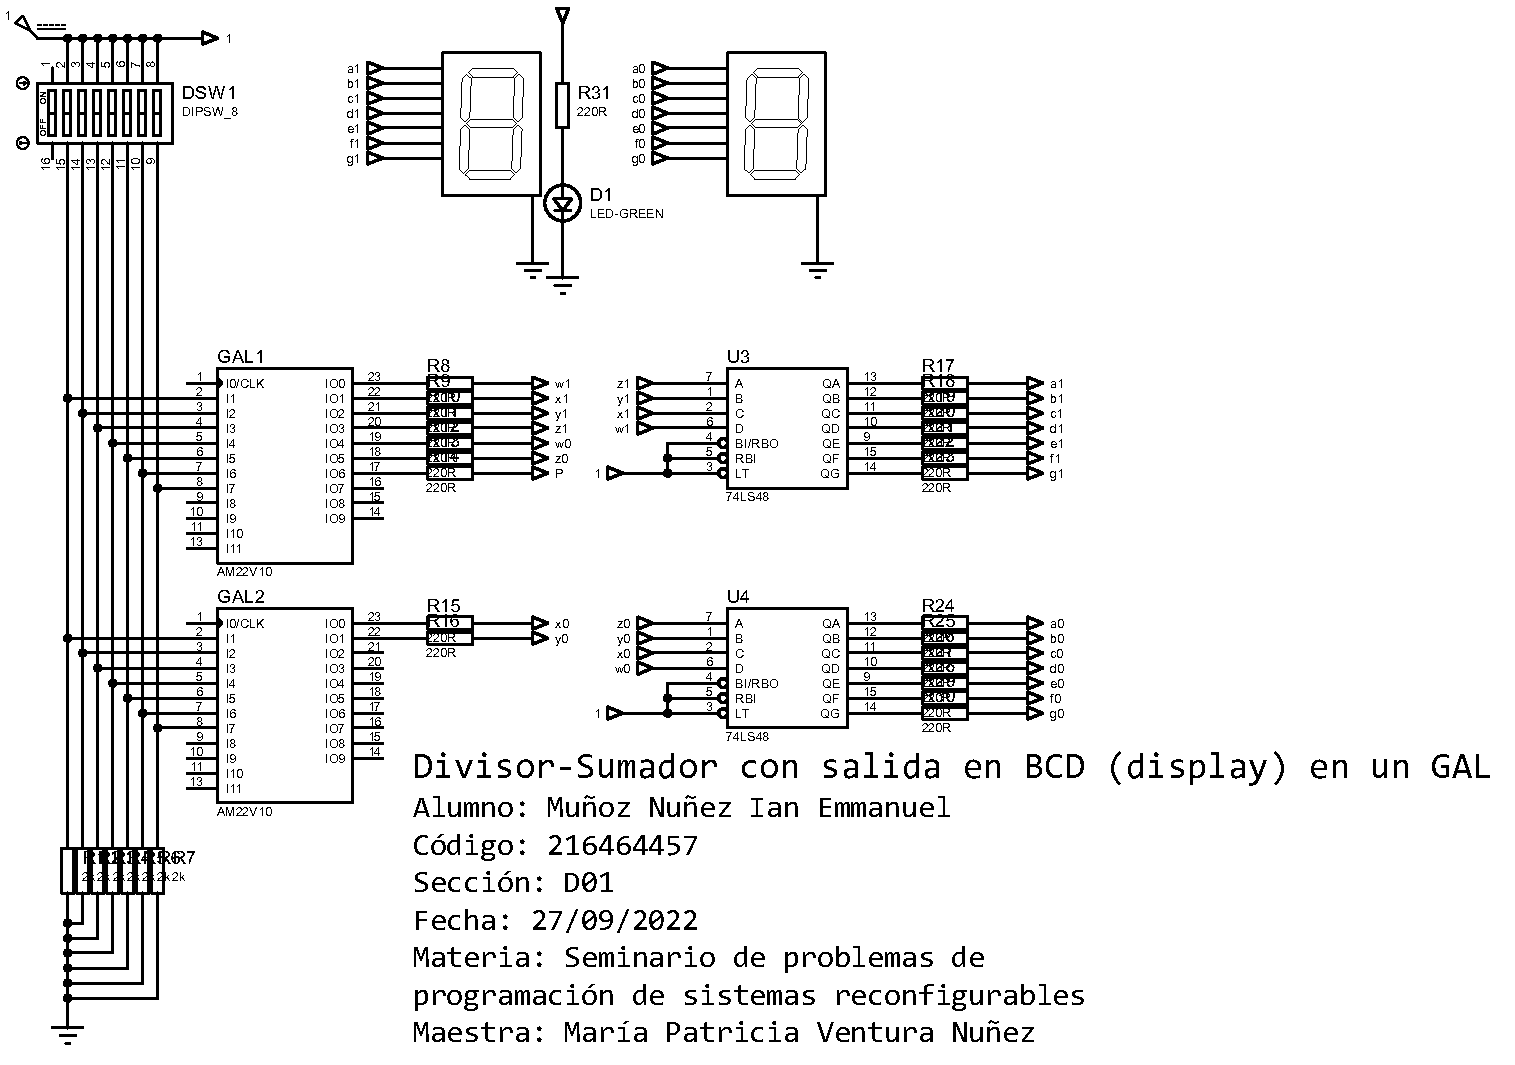
\includepdf[pages={1}]{main.PDF}

\newpage
\subsection{Protoboard}

\begin{figure}[h!]
    \centering
    \begin{subfigure}[tl]{0.45\textwidth}
        \centering
        \includegraphics[width=1\linewidth]{1662161142095.jpg}
    \end{subfigure}
    \begin{subfigure}[tr]{0.45\textwidth}
        \centering
        \includegraphics[width=1\linewidth]{1662161142120.jpg}
    \end{subfigure}
    \begin{subfigure}[bl]{0.45\textwidth}
        \centering
        \includegraphics[width=1\linewidth]{1662161142131.jpg}
    \end{subfigure}
    \begin{subfigure}[br]{0.45\linewidth}
        \centering
        \includegraphics[width=1\linewidth]{1662161142178.jpg}
    \end{subfigure}
    \caption{\sffamily Circuito en protoboard}
    \label{fig:proto}
\end{figure}

\section{Conclusión}
{\sffamily\Large
    \hspace{0.5cm} Considero que saber como funcionan los generadores de paridad es algo muy importante, pero hubo problemas al realizar el generador de paridad impar, pues la idea original era usar las compuertas lógicas \emph{xnor} para realizar el generador, pero se tuvieron problemas con estas, tanto las de la familia \emph{TTL} como de la \emph{CMOS}, por lo que mejor se decicidio usar compuertas \emph{xor} y solamente negar la salida del generador.
    
}

\end{document}
